\documentclass[varwidth=true, border=2pt]{standalone}
\usepackage{tikz}
\usetikzlibrary{patterns,calc,decorations.markings}

\begin{document}
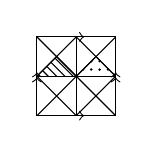
\begin{tikzpicture}
    \node (a) at (0,0) {};
    \node (b) at (1,0) {};
    \node (c) at (1,1) {};
    \node (d) at (0,1) {};
    \coordinate (m) at ($(a)!0.5!(c)$);
    \coordinate (ab) at ($(a)!0.5!(b)$);
    \coordinate (bc) at ($(b)!0.5!(c)$);
    \coordinate (cd) at ($(c)!0.5!(d)$);
    \coordinate (ad) at ($(a)!0.5!(d)$);
    \coordinate (left-intersection) at ($(m)!0.5!(d)$);
    \coordinate (right-intersection) at ($(m)!0.5!(c)$);
    \draw[pattern=north west lines] (ad.center) -- (left-intersection.center) -- (m.center);
    \draw[pattern=dots] (m.center) -- (right-intersection.center) -- (bc.center);
    \draw (a.center) -- (b.center) -- (c.center) -- (d.center) -- cycle;
    \draw (bc.center) -- (ad.center);
    \draw (cd.center) -- (ad.center);
    \draw (cd.center) -- (bc.center);
    \draw (ad.center) -- (ab.center);
    \draw (ab.center) -- (bc.center);
    \begin{scope}[decoration={
        markings,
        mark=at position 0.6 with {\arrow{>}}}
    ]
        \draw[postaction={decorate}] (a.center) -- (b.center);
        \draw[postaction={decorate}] (d.center) -- (c.center);
    \end{scope}

    \begin{scope}[decoration={
        markings,
        mark=at position 0.55 with {\arrow{>>}}}
    ]
        \draw[postaction={decorate}] (b.center) -- (c.center);
        \draw[postaction={decorate}] (a.center) -- (d.center);
    \end{scope}
    \draw (ab.center) -- (cd.center);
    \draw (a.center) -- (c.center);
    \draw (b.center) -- (d.center);
\end{tikzpicture}
\end{document}
